%% Source of figures/memory-flow.pdf (rules/04-figures-tables.md).
%% Build: xelatex -output-directory=figures figures/src/memory-flow.tex
%% Drawn from OpenTrading 0.5.1: src/core/runtime.ts (createMemory), src/core/memory/policy.ts, src/core/memory/binding/constraints.ts, src/core/memory/notebook/provider.ts, src/core/agent.ts (runTurn).
\documentclass[border=2pt]{standalone}
\usepackage{fontspec}
\IfFontExistsTF{Arial}{\setmainfont{Arial}}{\setmainfont{TeX Gyre Heros}}
\usepackage{tikz}
\usetikzlibrary{arrows.meta,fit,backgrounds}
\begin{document}
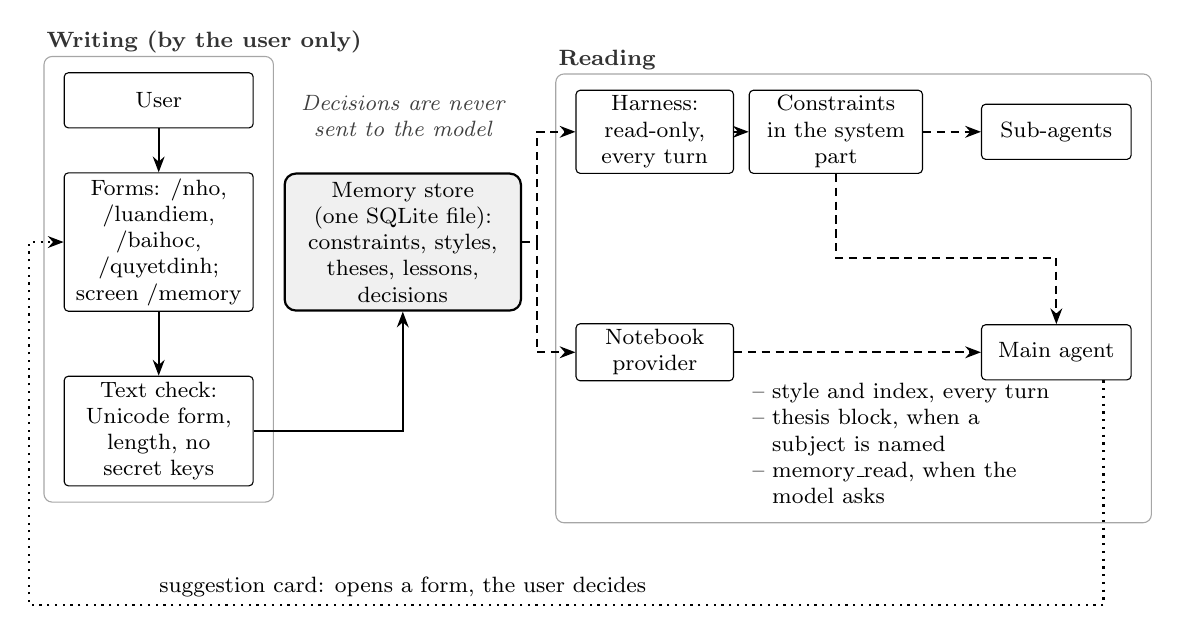
\begin{tikzpicture}[x=1mm, y=1mm,
  font=\fontsize{8}{9.5}\selectfont,
  box/.style={draw, rounded corners=1.5pt, align=center, inner sep=2pt, minimum height=7mm, fill=white},
  hub/.style={box, fill=gray!12, thick, rounded corners=4pt, minimum width=30mm, inner sep=3pt},
  wr/.style={-{Stealth[length=2mm]}, thick},
  rd/.style={-{Stealth[length=2mm]}, thick, dash pattern=on 3pt off 2pt},
  pr/.style={-{Stealth[length=2mm]}, thick, dotted},
  note/.style={align=center, inner sep=1pt, text=gray!50!black, font=\fontsize{8}{9.5}\selectfont\itshape},
  group/.style={draw, gray!70, rounded corners=3pt, inner xsep=2.5mm, inner ysep=2mm},
  glabel/.style={font=\fontsize{8}{9.5}\selectfont\bfseries, anchor=south west, gray!40!black, inner sep=1pt}
]
% Writing
\node[box, minimum width=24mm] (U) at (12,64) {User};
\node[box, minimum width=24mm] (F) at (12,46) {Forms: /nho,\\/luandiem,\\/baihoc,\\/quyetdinh;\\screen /memory};
\node[box, minimum width=24mm] (T) at (12,22) {Text check:\\Unicode form,\\length, no\\secret keys};
\draw[wr] (U) -- (F);
\draw[wr] (F) -- (T);

% Store
\node[hub] (S) at (43,46) {Memory store\\(one SQLite file):\\constraints, styles,\\theses, lessons,\\decisions};
\node[note] at (43,62) {Decisions are never\\sent to the model};
\draw[wr] (T.east) -- (43,22) -- (S.south);

% Reading, path (a): constraints
\node[box, minimum width=20mm] (H) at (75,60) {Harness:\\read-only,\\every turn};
\node[box, minimum width=22mm] (C) at (98,60) {Constraints\\in the system\\part};
\node[box, minimum width=19mm] (SA) at (126,60) {Sub-agents};
% Reading, path (b): notebook
\node[box, minimum width=20mm] (N) at (75,32) {Notebook\\provider};
\node[box, minimum width=19mm] (M) at (126,32) {Main agent};
\node[anchor=north west, align=left, text width=38mm, inner sep=1pt] (L) at (87,28.5)
  {-- style and index, every turn\\-- thesis block, when a\\\phantom{-- }subject is named\\-- memory\_read, when the\\\phantom{-- }model asks};

\draw[rd] (S.east) -- (60,46) |- (H.west);
\draw[rd] (60,46) |- (N.west);
\draw[rd] (H) -- (C);
\draw[rd] (C) -- (SA);
\draw[rd] (C.south) -- (98,44) -| (M.north);
\draw[rd] (N) -- (M);

% Proposal from the model
\draw[pr] ([xshift=6mm]M.south) -- ++(0,-28.5) -| (-4.5,46) -- (F.west);
\node[anchor=south, inner sep=1pt] at (43,0.5) {suggestion card: opens a form, the user decides};

% Groups
\begin{scope}[on background layer]
  \node[group, fit=(U)(F)(T)] (gw) {};
  \node[group, fit=(H)(C)(SA)(N)(M)(L)] (gr) {};
\end{scope}
\node[glabel] at (gw.north west) {Writing (by the user only)};
\node[glabel] at (gr.north west) {Reading};
\end{tikzpicture}
\end{document}
